\chapter{Algoritmo Genético}

El Algoritmo Genético (AG) es un método de computación evolutiva o \textit{machine learning}, basado en la teoría sintética de la evolución. Dicha teoría, a grandes rasgos, combina el mecanismo de la selección natural de Darwin con la genética de Mendel. Nos indica que el individuo más apto sobrevive, por lo que entre mejores sean los padres, mejor es la descendencia.

Actualmente el AG se utiliza para resolver problemas de búsqueda y optimización. Las áreas de aplicación son por ejemplo: economía, finanzas, medicina, ciencias sociales, investigación de operaciones, hidráulica, aeronáutica y química. Algunas aplicaciones en estas áreas son: diseño de redes de agua potable, optimización de portafolios de inversión, el problema del agente viajero y asignar asientos en un evento.

Los pasos que se siguen en el AG son los siguientes:

\begin{enumerate}
\item Selección: Se define una población inicial de tamaño $n$. De ésta se eligen 2 padres con los cuales se va a formar un hijo. La selección de los padres depende de qué tan aptos sean.

\item Cruce: Con cierta probabilidad se toma información de los padres. Dicha información la llamaremos genes.

\item Mutación: Cada gen agregado al hijo tiene una probabilidad pequeña de mutar.

\item Reemplazamiento: Se repiten los 3 pasos anteriores hasta formar $n$ hijos y poder reemplazar la población inicial.
\end{enumerate}

Con este proceso se obtiene una generación. El número de generaciones así como el tamaño de la población se pueden fijar antes de iniciar con el algoritmo. En la \figurename{~\ref{fig_AG}} podemos ver el diagrama de los pasos mencionados.

\begin{figure}[H]
\centering
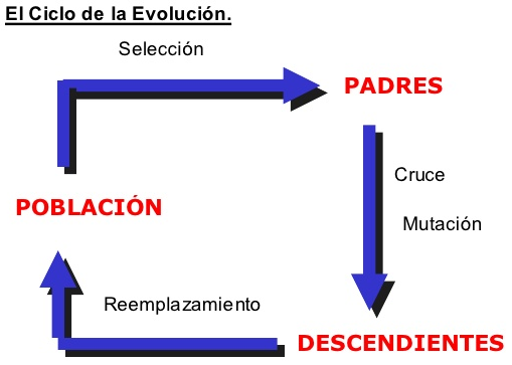
\includegraphics[scale = 0.45]{AG} %width=\textwidth
\caption{\textit{Algoritmo Genético}}\label{fig_AG}
\end{figure}

En la siguiente sección explicaremos cómo encontramos una buena asignación utilizando el AG. Cabe mencionar que Reeves y Rowe en su libro \textit{Genetic Algorithms: Principles and Perspectives} [\ref{ReevesRowe}], nos indican que se puede generar una nueva población haciendo el cruce y la mutación o utilizando sólo una de ellas. En nuestro caso, la estrategia que seguimos fue utilizar ambas.


%\section{Algoritmo Genético para obtener una buena asignación}
\section{Algoritmo Genético aplicado a los horarios}

El objetivo principal de este proyecto es obtener una matriz con la asignación final de materias, profesores y horas. Para ello haremos uso del AG. A continuación vamos a definir los términos que utilizaremos:

\begin{itemize}
\item[-] Asignación: Matriz de 3 columnas con la información de materias, profesores y horarios.

\item[-] Población: Conjunto de $n$ asignaciones.

\item[-] Padre: Asignación seleccionada, de la población, para formar un hijo.

\item[-] Gen: Vector de 3 entradas (Materia, Profesor, Horario) con la información extraída de una asignación.

\item[-] Hijo: Asignación formada a partir de los genes de 2 padres.

\item[-] Probabilidad de mutación: Debe de ser un valor pequeño. Definimos \textit{prob\_mutacion} $ = \dfrac{1}{24} \approx 0.04$

\item[-] Generación: Se dice que se tiene una generación cuando se ha repetido $n$ veces el proceso para crear un hijo y se puede reemplazar la población.
\end{itemize}

Los pasos que seguimos para obtener una buena asignación son los siguientes:

\begin{enumerate}
\item \textbf{Generar una población inicial}

Se generan $n$ asignaciones a partir del esqueleto simulado (ver Sección \ref{sec_esqueletos}) y de las solicitudes pseudo-reales simuladas (ver Sección \ref{SimSolicitudesProfesores}).

\item \textbf{Calificar cada asignación de la población}

Cada asignación tiene 2 tipos de calificaciones:

\begin{enumerate}
\item Por gen: Se califica cada gen de la asignación. Se premia con +5 si el profesor asignado es de tiempo completo. Se penaliza con -1 por cada asignación que pudo haber tenido un profesor de tiempo completo y tiene un profesor de asignatura. Para tener una calificación diferente para cada grupo, sumamos a cada gen una $\epsilon \in [0,0.1]$.

\item Global: Se califica la asignación completa. Se penaliza con -1 por cada grupo en el esqueleto sin profesor. Se penaliza con -10 por cada materia pedida por algún profesor de tiempo completo y no se le asignó. Se suma el promedio de las calificaciones por gen.

Nota:
Si el número máximo de asignaciones es 2 y un profesor pidió 3 o más  materias pero sólo se le asignó 1, entonces se penaliza una materia. Si se le asignaron, 2 no hay penalización.
\end{enumerate}

\item \textbf{Ordenar de acuerdo a la calificación}

Los genes de cada asignación se ordenan de menor a mayor calificación. Porque se quiere elegir con mayor probabilidad los genes con mejor calificación.

Las asignaciones se ordenan de menor a mayor calificación. Porque se quiere elegir con mayor probabilidad las asignaciones con mejor calificación.

\item \textbf{Elegir 2 padres}

Los padres se eligen con probabilidad: $\mathbb{P}(\text{elegir la asignación } i \text{ ya ordenada}) = \dfrac{2i}{n(n+1)}$, donde $i$ es la posición de la asignación con respecto a su calificación.

\item \textbf{Elegir un gen}

Primero de elige al azar un padre (ambos tienen probabilidad $\dfrac{1}{2}$). Una vez que se eligió un padre, seleccionar un gen: $\mathbb{P}(\text{elegir el gen } i \text{ ya ordenado}) = \dfrac{2i}{g(g+1)}$, donde $i$ es la posición del gen en la asignación con respecto a su calificación y $g$ es el número de genes que tiene la asignación.

\item \textbf{Mutación}

Se simula un número aleatorio, si ese número es menor a \textit{prob\_mutacion}, entonces el gen tiene una mutación. Si un gen muta, entonces se elige un gen de las solicitudes pseudo-reales y se intercambia por el gen previamente seleccionado.

\item \textbf{Agregar gen}

Una vez definido el gen, éste se agrega al hijo.

\item \textbf{Ajustar información}

Se quita la información en los padres, del profesor en el gen elegido, a esa hora y con esa materia. Ésto para evitar que se elijan genes repetidos para el hijo.

\item \textbf{Repetir 5 - 8}

Repetir los pasos 5 al 8 hasta que uno de los padres se quede sin genes.

\item \textbf{``Pegar'' genes}

``Pegar'' los genes restantes del otro padre al hijo.

%\item \textbf{Calificar hijo}
%
%Calificar los genes del hijo y ordenarlos de acuerdo a sus calificaciones.

\item \textbf{Repetir 4 - 10}

Repetir los pasos 4 al 10 $n$ veces para poder formar una generación.

\item \textbf{Reemplazar población}

Reemplazar a la población con la que se formó la generación.

\item \textbf{Repetir 2 - 12}

Repetir los pasos 2 al 12 hasta completar el número de generaciones deseadas.

\item \textbf{Asignación final}

Definir la asignación final como el hijo mejor calificado de la última generación.
\end{enumerate}


\begin{figure}[H]
\centering
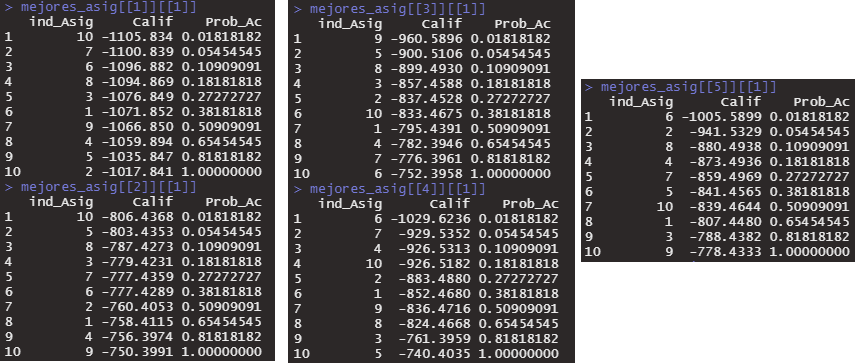
\includegraphics[width=\textwidth]{ej_calif_asignaciones} %scale = 0.7
\caption{\textit{Ejemplo con calificaciones de asignaciones}}
\end{figure}


Algunas notas que se deben de considerar en la asignación final:

\begin{itemize}
\item[-] Algunos profesores se les asignaron 2 cálculos

\item[-] Hay profesores que ya no imparten clases en la Facultad (nota en la sección de los profesores)

\item[-] 

\item[-] 
\end{itemize}